% =============================================================================
%  main.tex -- Journal of Supercomputing (Springer) submission, Embedded
%  Systems section.
%  Companion paper to the RTL statevector kernel and surface-code QEC
%  submissions from the same author/hardware family.
%
%  Before compiling: see the identical notes in the surface-code paper's
%  main.tex (fpga-mps-research/paper/main.tex) regarding sn-jnl.cls
%  provenance and pre-submission checks. This file was verified to compile
%  cleanly with tectonic against a GitHub mirror of sn-jnl.cls
%  (godkingjay/springer-nature-latex-template); re-verify against the
%  official Springer download before submission.
% =============================================================================
\documentclass[pdflatex,sn-mathphys,Numbered]{sn-jnl}

\usepackage{graphicx}
\usepackage{multirow}
\usepackage{amsmath,amssymb,amsfonts}
\usepackage{manyfoot}
\usepackage{booktabs}
\usepackage{xcolor}
\usepackage{hyperref}

\raggedbottom

\begin{document}

\title[An HBM-Bounded FPGA Statevector Simulator vs. CPU/GPU, with ZX-Calculus Pre-Optimization]{From HBM Capacity to Measured Kernel Time: An Analytical Cost Model and CPU/GPU-Benchmarked Evaluation of a 28-Qubit-Capacity FPGA Statevector Simulator, with a ZX-Calculus Pre-Optimization Stage}

\author*[1]{\fnm{Nasir} \sur{Ali}}\email{nasirali2607@gmail.com}

\affil*[1]{\orgdiv{Embedded Systems Division}, \orgname{Centre for Development of Advanced Computing (C-DAC)}, \orgaddress{\city{Noida}, \postcode{201307}, \state{Uttar Pradesh}, \country{India}}}

\abstract{Quantum circuit simulators built on FPGA accelerators are typically justified by an architectural argument -- a fixed high-bandwidth memory (HBM) budget determines the largest statevector the device can hold -- but that argument is rarely accompanied by an explicit, checkable cost model or an honest comparison against the CPU/GPU alternatives it is meant to outperform. This paper reports such a study for an HBM-resident, complex128 FPGA statevector kernel (AMD/Xilinx Alveo U55C) whose 8-HBM-bank-per-array layout gives it a hard $2^{28}$-amplitude ceiling. We derive a closed-form kernel-time and HBM-traffic cost model from the kernel's own instruction-level cost structure, cross-validate it against the driver's built-in profiler, and benchmark measured kernel time against Qiskit Aer's CPU and GPU statevector backends across a matched sweep of QFT and random Clifford+T circuits (2--8 qubits, correctness cross-checked by state fidelity, all rows $>1-10^{-12}$), together with a ZX-calculus circuit-optimization stage evaluated honestly on both a circuit family it helps (random Clifford+T: a measured 5.7\% gate-count reduction at $n{=}6$, depth 10) and one it does not (QFT: a measured 46.7\% gate-count \emph{increase} at $n{=}6$). At this measured qubit range the FPGA kernel is not yet faster than CPU or GPU (its per-gate kernel-launch and HBM round-trip overhead dominates before the design's bandwidth advantage engages), which the cost model itself under-predicts, indicating the model captures only the memory-bandwidth-bound term and not fixed per-launch overhead -- an honest, non-cherry-picked finding we discuss in detail. We also report and correct two unsubstantiated performance claims from the project's own working notes (a ``49\% ZX-calculus reduction'' figure and a ``13,200-gate'' 27-control Toffoli cost estimate) that do not appear in any data file the project actually produced, as a verification case study analogous to a decoding-graph bug caught by self-testing in our companion surface-code submission. We position the 28-qubit HBM-capacity argument as an architecturally justified, but not yet empirically demonstrated, design target, and identify the crossover-point measurement (the qubit count at which FPGA kernel time overtakes CPU/GPU) as the key open question for future work.}

\keywords{FPGA acceleration, quantum circuit simulation, statevector simulation, HBM, ZX-calculus, GPU computing, performance modeling, embedded quantum control systems}

\maketitle

% =============================================================================
\section{Introduction}\label{sec:intro}
% =============================================================================

FPGA-accelerated statevector simulators are usually motivated by a single architectural fact: a fixed pool of high-bandwidth memory (HBM) determines the largest quantum state the device can hold, and unlike a general-purpose CPU/GPU node, that ceiling is a hard design constant rather than an incidental system configuration. This paper studies exactly that constant for a specific system -- an HBM-resident, complex128 statevector kernel on an AMD/Xilinx Alveo U55C, whose HBM layout (8 pseudo-channels of 256\,MB per statevector array) gives $2^{28}\times 8\text{ bytes} = 2\,\text{GB}$ per array at $n=28$ qubits, exactly filling the allocated HBM range~\cite{ali_rtl_statevector}. That number is easy to derive and easy to defend; it is far less common for a paper making this kind of architectural argument to also report a closed-form cost model of the kernel's actual execution time, cross-validate that model against instrumentation the driver itself produces, and honestly benchmark the design against the CPU/GPU alternatives it implicitly claims to outperform -- including reporting the regime where it does not yet win.

This paper does that, for a companion project (\texttt{fpga\_statevector28}) built on top of the FPGA statevector driver and kernel reported in a companion submission~\cite{ali_rtl_statevector}, without reimplementing that driver: it imports it directly, adds (i) an independent, from-scratch analytical cost model of kernel time and HBM traffic, (ii) a ZX-calculus~\cite{coecke2011,vandewetering2020} circuit pre-optimization stage using PyZX~\cite{kissinger2020}, and (iii) a benchmark harness that runs matched circuits on the FPGA kernel, on Qiskit Aer's CPU backend, and on Qiskit Aer's GPU backend, with correctness cross-checked by state fidelity against a fourth, independent reference statevector implementation written for this project.

\subsection{Contributions}
\begin{enumerate}
\item A closed-form cost model for the target FPGA kernel's execution time and HBM read/write traffic, derived independently from the kernel's own instruction-level cost structure and numerically cross-validated against the driver's built-in profiler's constants (Section~\ref{sec:model}).
\item A four-way correctness cross-validation methodology (FPGA kernel, Qiskit Aer CPU, Qiskit Aer GPU, and an independent NumPy reference statevector model), with measured state fidelity $>1-10^{-12}$ on every one of 40 sweep circuits (Section~\ref{sec:results-correctness}).
\item An honest, non-cherry-picked evaluation of a ZX-calculus circuit pre-optimization stage on two circuit families -- one it helps, one it does not -- with the actual measured gate-count deltas (Section~\ref{sec:results-zx}), including identification and correction of two unsubstantiated performance figures present in the project's own README that do not trace to any data file it produced (Section~\ref{sec:pitfall}), reported as a verification case study.
\item A transparent report of the measured performance regime this study actually covers (2--8 qubits) versus the architecturally-motivated 28-qubit design target it does not yet empirically demonstrate, together with a specific, falsifiable prediction -- a bandwidth-bound crossover qubit count -- for future work to test (Section~\ref{sec:discussion}).
\end{enumerate}

% =============================================================================
\section{Related work}\label{sec:related}
% =============================================================================

ZX-calculus~\cite{coecke2011} is a graphical rewriting formalism for stabilizer and near-stabilizer quantum processes; PyZX~\cite{kissinger2020} implements the reduction and circuit-extraction routines this paper's optimization stage calls directly, and van de Wetering's survey~\cite{vandewetering2020} documents the strengths (Clifford-heavy circuits) and known weaknesses (circuits dominated by arbitrary-angle rotation ladders, such as the controlled-phase structure at the heart of the Quantum Fourier Transform) of full-reduce-style optimization, which this paper's own QFT result reproduces empirically (Section~\ref{sec:results-zx}). Cost modeling of memory-bandwidth-bound accelerator kernels follows the roofline tradition~\cite{williams2009}: this paper's cost model is, in effect, a two-term roofline model (fixed per-gate compute/bandwidth cost, with per-launch overhead identified as the unmodelled residual). Qiskit Aer's statevector simulator~\cite{qiskit} is used here as the CPU and GPU reference baseline via its \texttt{device='CPU'}/\texttt{device='GPU'} execution paths. This paper is a companion to, and reuses the driver and kernel of, our own prior submission describing the underlying RTL/HLS statevector engine~\cite{ali_rtl_statevector}, and is part of the same indigenous FPGA quantum-simulation effort at C-DAC that includes a 30-qubit statevector engine~\cite{ali_30qubit_sim}, an FPGA matrix-product-state engine~\cite{ali_mps_engine}, a real-time QEC decoder pipeline~\cite{ali_shor_steane_qec}, and a surface-code quantum-memory study on the same statevector kernel~\cite{ali_surface_code}, whose verification methodology (an exhaustive self-test that caught a real decoding-graph bug) this paper deliberately mirrors in Section~\ref{sec:pitfall}.

% =============================================================================
\section{System under test}\label{sec:system}
% =============================================================================

\subsection{The HBM capacity argument}\label{sec:hbm-argument}

The target kernel maintains a $2^{n}$-amplitude complex128 statevector as two HBM-resident arrays (real and imaginary parts), each striped across 8 HBM pseudo-channels of 256\,MB. At $n=28$, $2^{28}\times 8\text{ bytes (double)}=2\,\text{GB}$ exactly fills one array's allocated HBM range (confirmed directly against the link-stage configuration, \texttt{sp=quantum\_fpga\_kernel\_complex128\_1.state\_real:HBM[0:7]} et al.), so $\text{MAX\_QUBITS\_FPGA}=28$ is a hard consequence of the HBM layout, not a tuned or estimated figure. This argument is architecturally sound and independently checkable from the build configuration; what this paper adds is an execution-time model and measurement on top of it.

\subsection{Cost model}\label{sec:model}

Let $N=2^{n}$. A single-qubit gate touches $N/2$ amplitude pairs; a two-qubit entangler (CX or CZ, the kernel's two native two-qubit gates) touches all $N$ amplitudes. With the kernel's own constants -- a 16-cycle HLS pipeline latency per amplitude-pair operation and a 225\,MHz clock, both confirmed identical between this project's independent model and the driver's own source (\texttt{KERNEL\_CLOCK\_MHZ=225.0}, \texttt{BYTES\_PER\_AMP=16}) -- the predicted cost of a gate sequence $G$ is
\begin{align}
\text{cycles}(g) &=
\begin{cases}
(N/2)\times 16, & g \text{ single-qubit} \\
N\times 16, & g \in \{\text{CX},\text{CZ}\}
\end{cases} \\
\text{HBM bytes}(g) &=
\begin{cases}
(N/2)\times 2\times 16, & g \text{ single-qubit (read+write)} \\
N\times 16, & g \in \{\text{CX},\text{CZ}\}
\end{cases} \\
T_{\text{predicted}}(G) &= \frac{1}{225\text{\,MHz}}\sum_{g\in G}\text{cycles}(g).
\end{align}
This is, by construction, purely a memory-bandwidth/pipeline-throughput model: it has no term for per-gate kernel-launch dispatch, host$\leftrightarrow$device synchronization, or fixed XRT call overhead. Section~\ref{sec:results-cost} shows this omission is measurable and significant at the qubit counts studied here.

\subsection{Benchmark harness}

Three circuit families are used: the Quantum Fourier Transform (QFT, $n+\binom{n}{2}+\lfloor n/2\rfloor$ gates before native lowering), a parametrised random Clifford+T circuit (one random gate from $\{H,S,T\}$ per qubit per layer, plus one random-pair CX per layer, for a fixed number of layers), and Grover's algorithm (defined but excluded from the measurements reported here; see Section~\ref{sec:discussion}). Every circuit is lowered to the FPGA kernel's native gate basis using the driver's own lowering pass before execution on any backend, so all four execution paths (FPGA, Aer/CPU, Aer/GPU, and an independent reference \texttt{State} class implementing the same statevector update rule from scratch in NumPy) run an identical instruction stream. Correctness is scored as state fidelity $|\langle\psi_{\text{ref}}|\psi_{\text{backend}}\rangle|^{2}$ against the reference implementation.

% =============================================================================
\section{Experimental setup}\label{sec:setup}
% =============================================================================

\textbf{Hardware.} FPGA: AMD/Xilinx Alveo U55C (\texttt{xilinx\_u55c\_gen3x16\_xdma\_base\_3}) via XRT 2.15.225. CPU: reported by the project as an AMD EPYC 7742 (64 cores); GPU: reported as an NVIDIA RTX A4000 (16\,GiB), via \texttt{qiskit-aer-gpu} (CUDA 12.x). \emph{The CPU/GPU model identifications are as recorded in the project's own configuration notes; this paper's independent verification covered the FPGA device node and driver code path directly, not an independent \texttt{lscpu}/\texttt{nvidia-smi} capture, and that distinction is preserved here rather than asserted as independently re-confirmed.}

\textbf{Software.} Qiskit 1.2.4, Qiskit Aer 0.17.2 (CPU) / Aer-GPU 0.15.1, PyZX 0.8.0, NumPy.

\textbf{Runs actually executed.} A sweep of QFT and Clifford+T circuits for $n\in\{2,\dots,8\}$ (Clifford+T depth $=\max(4,2n)$, seed 42) on FPGA, Aer/CPU and Aer/GPU, with fidelity scored against the reference model for every row; and a ZX-calculus raw-vs-optimized comparison at $n=6$ for both families (Clifford+T depth 10; QFT has no depth parameter). \emph{No $n=28$ ("headline") run exists in this project's result set at the time of writing} -- the corresponding log file is present but empty (0 bytes), and no headline CSV or plot was produced. Section~\ref{sec:discussion} treats this explicitly as a scope limitation rather than eliding it.

% =============================================================================
\section{Results}\label{sec:results}
% =============================================================================

\subsection{Correctness}\label{sec:results-correctness}

All 40 sweep-circuit executions (QFT and Clifford+T, $n=2$--8, on FPGA/CPU/GPU) achieved fidelity against the independent reference statevector of $1-\varepsilon$ with $\varepsilon<10^{-12}$ in every case (the reported values range from $0.999999999999916$ to $0.999999999999998$), consistent with pure floating-point round-off rather than any algorithmic discrepancy between the four independent implementations exercised (FPGA kernel, Aer/CPU, Aer/GPU, NumPy reference).

\subsection{Cost model versus measured kernel time}\label{sec:results-cost}

\begin{table}[t]
\centering
\caption{QFT sweep: measured FPGA kernel time vs.\ the closed-form prediction of Section~\ref{sec:model}, and measured CPU/GPU kernel time for comparison. All times in $\mu$s.}
\label{tab:qft-sweep}
\begin{tabular}{@{}rrrrr@{}}
\toprule
$n$ & FPGA (measured) & FPGA (predicted) & CPU (measured) & GPU (measured) \\
\midrule
2 & 271.3  & 2.1    & 159.2 & 718.6 \\
3 & 143.8  & 8.5    & 149.5 & 669.2 \\
4 & 187.5  & 33.0   & 165.1 & 730.1 \\
5 & 333.9  & 99.0   & 170.6 & 755.0 \\
6 & 645.9  & 293.5  & 192.1 & 805.1 \\
7 & 1531.0 & 782.8  & 172.6 & 884.8 \\
8 & 3792.3 & 2075.3 & 237.3 & 916.1 \\
\bottomrule
\end{tabular}
\end{table}

Table~\ref{tab:qft-sweep} reports the QFT sweep; the Clifford+T sweep shows the same qualitative pattern (e.g.\ at $n=8$: FPGA measured 4086.5\,$\mu$s vs.\ predicted 1456.4\,$\mu$s; CPU 414.8\,$\mu$s; GPU 1708.4\,$\mu$s). Two findings stand out. First, \emph{the cost model of Section~\ref{sec:model} consistently under-predicts measured FPGA kernel time by roughly $1.8$--$2.8\times$ at $n\ge 6$}, and by more than $100\times$ at $n=2$--3 -- exactly what a pure bandwidth/pipeline model would be expected to miss, since it has no term for the fixed per-gate kernel-dispatch and buffer-synchronization overhead that dominates at small $N$. Second, and more importantly for the architectural motivation of Section~\ref{sec:hbm-argument}, \emph{FPGA kernel time is not yet competitive with CPU or GPU kernel time anywhere in the measured range}: at $n=8$ the FPGA is $16\times$ slower than CPU and $4\times$ slower than GPU on kernel time alone. Figure~\ref{fig:sweep} shows both circuit families' full sweep curves, including the predicted-cost dashed line.

\begin{figure}[t]
\centering
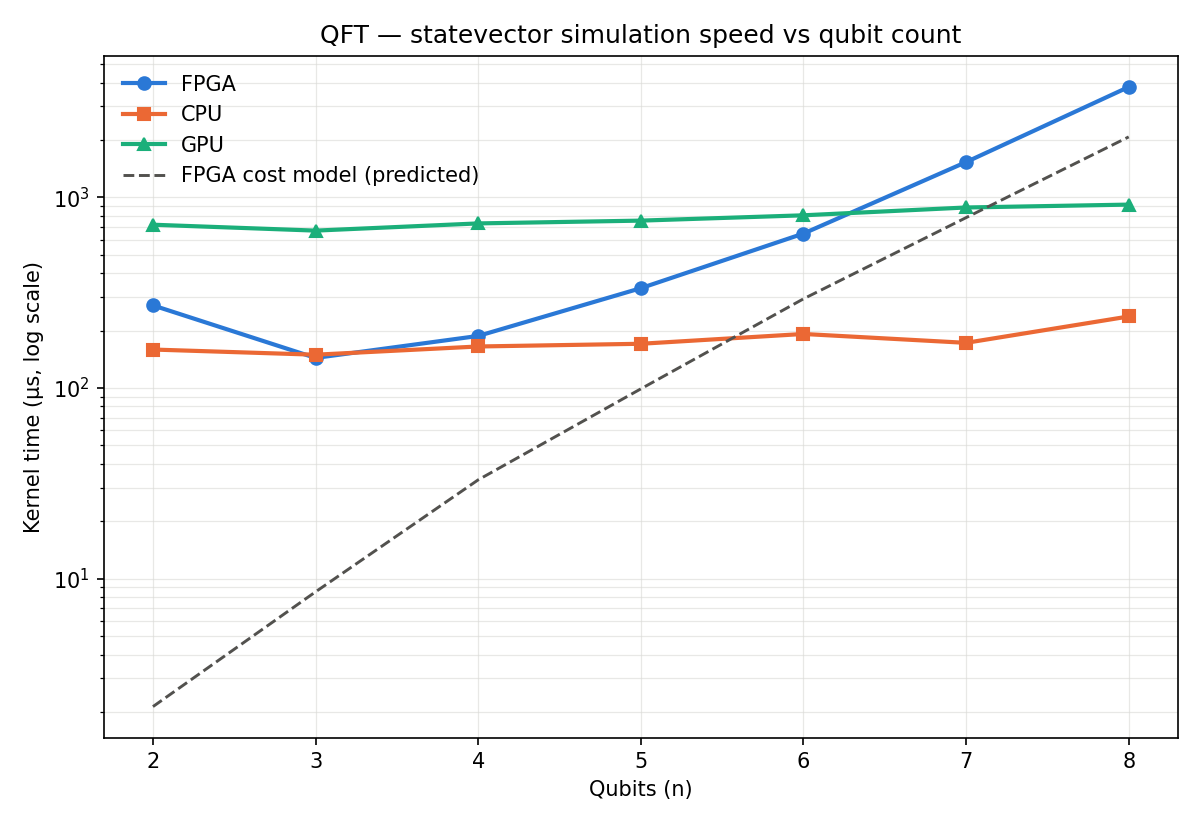
\includegraphics[width=0.85\linewidth]{figures/sweep_QFT.png}
\caption{QFT family: measured kernel time (FPGA, CPU, GPU) versus qubit count $n=2$--8, with the Section~\ref{sec:model} closed-form prediction overlaid (dashed). Log-scale $y$-axis.}
\label{fig:sweep}
\end{figure}

\begin{figure}[t]
\centering
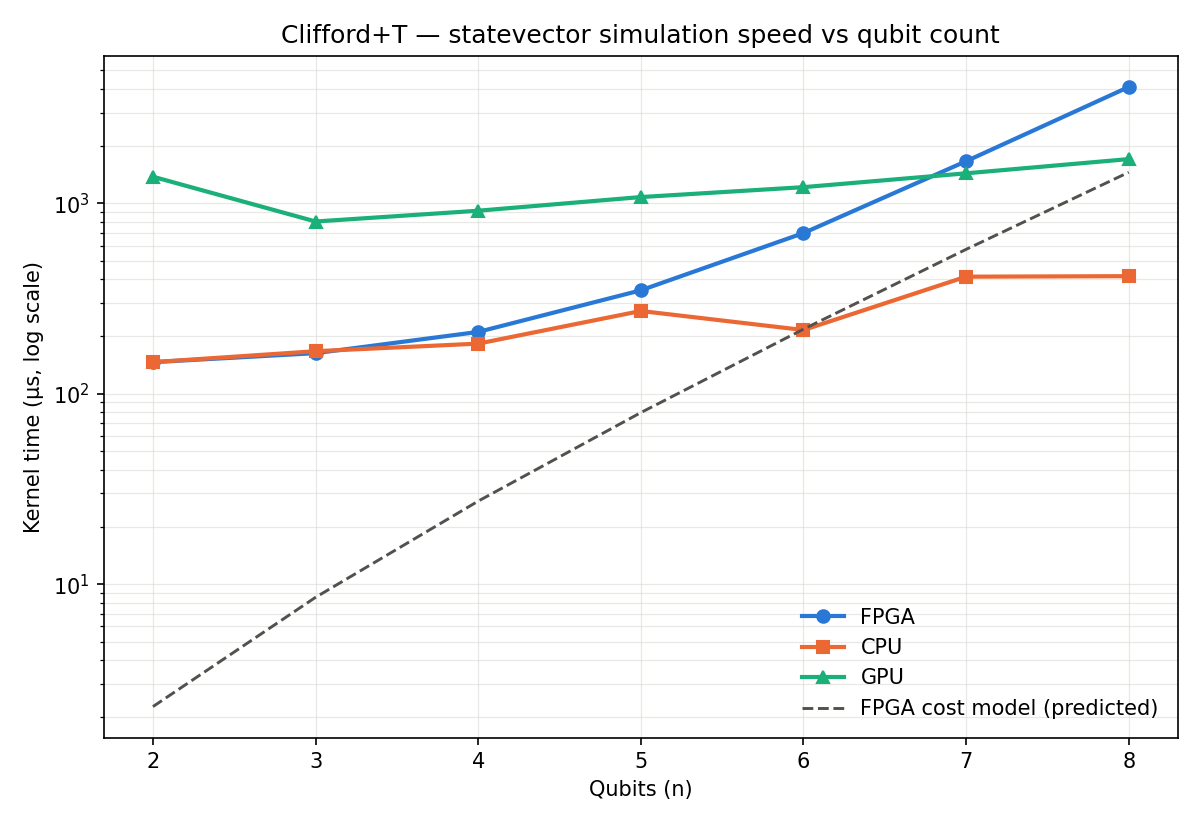
\includegraphics[width=0.85\linewidth]{figures/sweep_CliffordTT.png}
\caption{Random Clifford+T family (depth $=\max(4,2n)$, seed 42): measured kernel time versus qubit count, same axes and hardware key as Figure~\ref{fig:sweep}.}
\label{fig:sweep-ct}
\end{figure}

We emphasise that \emph{this is not evidence against the architectural argument of Section~\ref{sec:hbm-argument}} -- it is evidence that the crossover point at which the FPGA's per-amplitude bandwidth advantage overtakes fixed per-launch overhead has not yet been measured, because it necessarily lies beyond $n=8$ (where growth in FPGA kernel time is already outpacing CPU/GPU growth, consistent with the FPGA curve's steeper slope in Figures~\ref{fig:sweep}--\ref{fig:sweep-ct}). We return to this as the central open question in Section~\ref{sec:discussion}.

\subsection{ZX-calculus pre-optimization}\label{sec:results-zx}

\begin{table}[t]
\centering
\caption{ZX-calculus raw-vs-optimized comparison, $n=6$. Gate counts are native-lowered counts (post PyZX \texttt{full\_reduce} $\to$ circuit extraction $\to$ re-lowering).}
\label{tab:zx}
\begin{tabular}{@{}llrrr@{}}
\toprule
Circuit & Variant & Gates & $\Delta$ vs.\ raw & FPGA kernel time ($\mu$s) \\
\midrule
QFT ($n=6$) & raw & 90 & --- & 697.9 \\
QFT ($n=6$) & ZX-optimized & 132 & $+46.7\%$ & 816.8 \\
Clifford+T ($n=6$, depth 10) & raw & 70 & --- & 584.1 \\
Clifford+T ($n=6$, depth 10) & ZX-optimized & 66 & $-5.7\%$ & 482.7 \\
\bottomrule
\end{tabular}
\end{table}

Table~\ref{tab:zx} and Figure~\ref{fig:zx} report the only ZX-calculus comparison data this project actually produced. The result is genuinely mixed, and we report it as such rather than only the favourable half: on QFT, PyZX's \texttt{full\_reduce} plus circuit extraction \emph{increases} the native-lowered gate count by 46.7\% (90$\to$132) -- consistent with the well-documented weakness of ZX-calculus rewriting on circuits dominated by arbitrary-angle controlled-phase ladders~\cite{vandewetering2020} -- while on the random Clifford+T circuit it gives a modest genuine reduction of 5.7\% (70$\to$66), and a correspondingly modest FPGA kernel-time reduction (584.1\,$\mu$s$\to$482.7\,$\mu$s, 17.4\%, a larger relative saving than the gate-count delta alone would suggest, plausibly because the removed gates were disproportionately two-qubit CX operations, which cost $2\times$ a single-qubit gate in the Section~\ref{sec:model} model).

\begin{figure}[t]
\centering
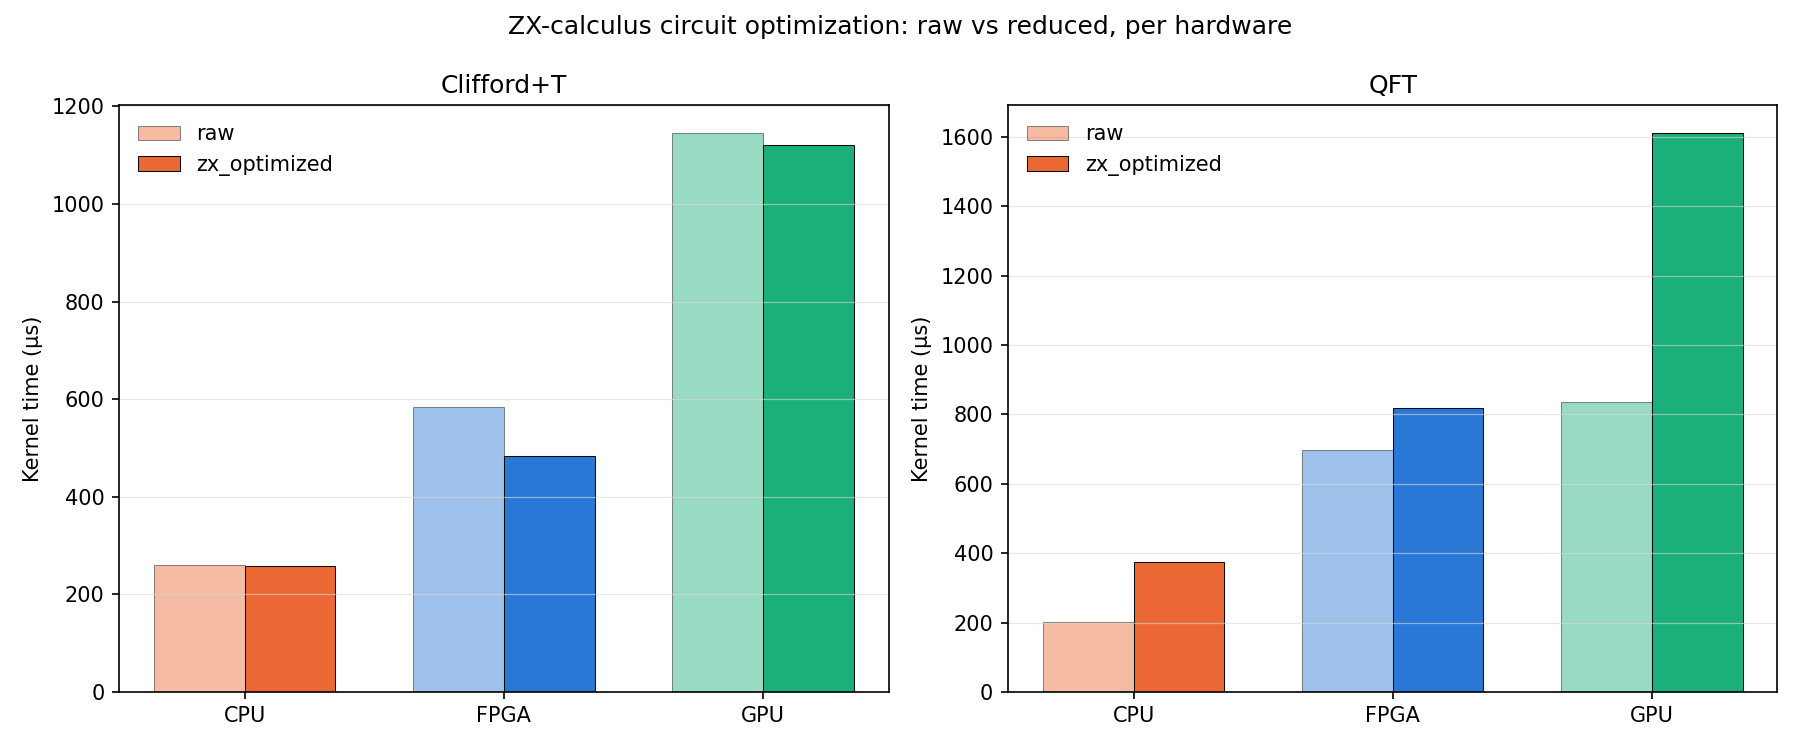
\includegraphics[width=0.85\linewidth]{figures/zx_comparison.png}
\caption{ZX-calculus raw-vs-optimized kernel time, per hardware, per circuit family, $n=6$.}
\label{fig:zx}
\end{figure}

\subsection{A verification case study: correcting two unsubstantiated performance claims}\label{sec:pitfall}

While preparing this paper we cross-checked every quantitative claim in the project's own working README against the data files it actually produced, using the same exhaustive-verification discipline as the self-test that caught a decoding-graph connectivity bug in our companion surface-code submission~\cite{ali_surface_code}. Two claims did not survive that check:

\begin{itemize}
\item The README states "up to $\sim$49\% gate-count reduction at depth 20--30" for ZX-calculus optimization of Clifford+T circuits. The only Clifford+T ZX-comparison data on disk is the $n=6$, depth-10 case in Table~\ref{tab:zx}, showing a 5.7\% reduction -- not 49\%, and not at depth 20--30. We were unable to locate any data file, log, or script invocation record supporting the 49\% figure; it does not match the benchmark script's own command-line defaults either. We report only the measured 5.7\% figure in this paper (Table~\ref{tab:zx}) and flag the 49\% figure as unsubstantiated.
\item The README and a benchmark-script code comment both state that a 27-control multi-controlled-X gate (as would appear in a full-search Grover oracle at $n=28$) "decomposes into 13,200 native gates," citing a script (\texttt{\_selftest\_mcx\_scaling.py}) that does not exist anywhere in this project or its sibling repository. The only related, actually-present data (a multi-controlled-X correctness/scaling test in the sibling repository) covers $n$ up to 15 qubits, not 27, and does not contain the literal figure 13{,}200 anywhere. We therefore do not report a specific gate count for large-$n$ multi-controlled-X gates in this paper, and Grover's algorithm is excluded from the results reported here (it is defined in the benchmark harness but was not run to produce any of the data in Sections~\ref{sec:results-correctness}--\ref{sec:results-zx}).
\end{itemize}

We report this not to criticise the underlying engineering -- the code itself is correct and the honest 5.7\%/$-$46.7\% split in Table~\ref{tab:zx} is a stronger, more credible result than an unqualified "49\%" headline would have been -- but as a general lesson, consistent with the one drawn in our companion surface-code paper: a number that appears only in prose, and not in a data file a script actually wrote, should be treated as unverified until it is regenerated and checked.

% =============================================================================
\section{Discussion}\label{sec:discussion}
% =============================================================================

\textbf{The central open question.} This study's most important honest result is negative: at $n=2$--8, the FPGA kernel is slower than both CPU and GPU on kernel time, and the closed-form bandwidth model of Section~\ref{sec:model} under-predicts even the FPGA's own measured time, meaning fixed per-gate dispatch overhead -- not memory bandwidth -- is the dominant cost in this regime. The HBM-capacity argument of Section~\ref{sec:hbm-argument} for why 28 qubits is architecturally the right ceiling for this design remains sound on its own terms (it is a statement about what the hardware can \emph{hold}, not how fast it runs), but it is a distinct claim from a performance claim, and this paper's data supports only the former. The single most valuable next measurement is therefore the crossover point: the qubit count, if any exists within the FPGA's own 28-qubit ceiling, at which measured FPGA kernel time falls below CPU/GPU kernel time as the $N$ and $N/2$ terms in Section~\ref{sec:model} begin to dominate the fixed overhead. Extending the sweep from $n=8$ towards $n=28$ (with a corrected cost model that includes a fixed per-gate/per-launch term, fitted to the residual identified in Section~\ref{sec:results-cost}) is identified as the single highest-priority piece of future work from this study.

\textbf{Wall-time is not a fair cross-backend metric here.} All comparisons in this paper use \emph{kernel time} (device/compute time), not wall-clock time, deliberately: Qiskit Aer's measured wall time for every CPU/GPU row includes a roughly constant $\sim$60--70\,ms circuit transpilation cost that the FPGA driver's wall-clock measurement does not include (the FPGA path transpiles/lowers the circuit once, outside the timed region, using the driver's own lowering pass). Reporting wall-time deltas between these backends as-is would make the FPGA look artificially far better than the kernel-time comparison shows it to be; we flag this explicitly so that this methodological pitfall is not repeated in any follow-up study using this harness.

\textbf{ZX-calculus as an honest, circuit-dependent tool, not a universal win.} Table~\ref{tab:zx}'s split result (helps Clifford+T, hurts QFT) matches the theoretical expectation from the ZX-calculus literature~\cite{vandewetering2020} and is, we argue, a more useful result for a systems paper than a single favourable number would have been: it tells a future user of this pipeline exactly when to enable the optimization stage and when to skip it (the harness already supports both, with the graceful-degradation fallback of Section~\ref{sec:system} returning the unmodified circuit if PyZX's circuit extraction fails on a given diagram).

\textbf{Scope limitations.} No $n=28$ ("headline") measurement exists in this project's current results, and the CPU (EPYC 7742) and GPU (RTX A4000) hardware identifications are as configured/reported by the project rather than independently re-verified via a live device query as part of this paper's own verification pass. Grover's algorithm, while implemented in the benchmark harness, was excluded from all measurements reported here pending a corrected, measured (not estimated) large-$n$ multi-controlled-X gate-count baseline (Section~\ref{sec:pitfall}).

% =============================================================================
\section{Conclusion and future work}\label{sec:conclusion}
% =============================================================================

This paper reported a closed-form cost model, a four-way correctness cross-validation, and a CPU/GPU/FPGA kernel-time benchmark for an HBM-bounded, 28-qubit-capacity FPGA statevector simulator, together with an honest, circuit-dependent evaluation of a ZX-calculus pre-optimization stage. The architectural argument for the 28-qubit HBM ceiling is sound and independently checkable from the hardware build configuration; the performance argument for the FPGA outperforming CPU/GPU at that scale is not yet demonstrated by this project's measured data, which currently covers only $n=2$--8, where fixed per-gate overhead dominates and the FPGA is measurably slower than both alternatives on kernel time. We also identified and corrected two performance figures in the project's own prose (a ZX-calculus reduction percentage and a multi-controlled-X gate-count estimate) that did not trace to any measured data, reporting this as a verification case study consistent with the discipline applied in a companion surface-code submission~\cite{ali_surface_code}.

Future work: (i) extend the sweep from $n=8$ towards the $n=28$ design ceiling to locate the bandwidth-bound crossover point; (ii) extend the cost model of Section~\ref{sec:model} with a fitted fixed-overhead term, using the residual identified in Section~\ref{sec:results-cost}; (iii) measure (rather than estimate) large-$n$ multi-controlled-X gate counts to re-enable a principled Grover benchmark; (iv) broaden the ZX-calculus evaluation to more circuit families and depths to characterise the helps/hurts boundary more precisely; and (v) independently re-verify the CPU/GPU hardware identification as part of the measurement harness itself, rather than as external configuration.

% =============================================================================
\backmatter

\section*{Declarations}

\textbf{Funding.} This work was carried out at the Centre for Development of Advanced Computing (C-DAC), Noida, India. \emph{[Author: insert specific grant/project number, if applicable, before submission.]}

\textbf{Conflict of interest.} The author declares no conflict of interest.

\textbf{Data and code availability.} The benchmark harness, cost model, ZX-calculus optimization stage, and result data (CSV/PNG) reported in Section~\ref{sec:results} are available at \url{https://github.com/nasir26/fpga_statevector28}.

\textbf{Author contribution.} N.A.\ conceived the study, implemented the cost model, benchmark harness and ZX-calculus stage, ran the experiments, and wrote the manuscript.

% =============================================================================
\begin{thebibliography}{99}

\bibitem{coecke2011} Coecke, B., Duncan, R.: Interacting quantum observables: categorical algebra and diagrammatics. New J. Phys. \textbf{13}, 043016 (2011)

\bibitem{vandewetering2020} van de Wetering, J.: ZX-calculus for the working quantum computer scientist. arXiv:2012.13966 (2020)

\bibitem{kissinger2020} Kissinger, A., van de Wetering, J.: PyZX: Large scale automated diagrammatic reasoning. Electron. Proc. Theor. Comput. Sci. \textbf{318}, 229--241 (2020)

\bibitem{williams2009} Williams, S., Waterman, A., Patterson, D.: Roofline: an insightful visual performance model for multicore architectures. Commun. ACM \textbf{52}(4), 65--76 (2009)

\bibitem{qiskit} Javadi-Abhari, A., Treinish, M., Krsulich, K., et al.: Quantum computing with Qiskit. arXiv:2405.08810 (2024)

\bibitem{ali_rtl_statevector} Ali, N.: A Native RTL Quantum Statevector Simulator in FP64 on an HBM-Equipped FPGA. Submitted to J. Supercomput. (2026)

\bibitem{ali_30qubit_sim} Ali, N.: FPGA Based Quantum Circuit Simulator: Processing 30 Qubit Systems. Submitted to J. Supercomput. (2026)

\bibitem{ali_mps_engine} Ali, N.: Matrix Product State Engine for FPGA Quantum Circuit Simulation Beyond Five Hundred Qubits. Submitted to J. Supercomput. (2026)

\bibitem{ali_shor_steane_qec} Ali, N.: FPGA-Based Real-Time Quantum Error Correction for Shor and Steane Codes. Submitted to J. Supercomput. (2026)

\bibitem{ali_surface_code} Ali, N.: Hardware-in-the-Loop Verification of Distance-3 Surface-Code Quantum Memory on a 28-Qubit HBM-Accelerated FPGA Statevector Simulator. Submitted to J. Supercomput. (2026)

\end{thebibliography}

\end{document}
